\section{Degree-distribution properties}
For each node $i$ in a undirected network, we can define its \emph{degree} $k_i$ as the number of edges connected to it. Formally, if $A$ is the adjacency matrix of the network, we define:
\begin{equation*}
    k_i = \sum_j A_{ij}.
\end{equation*}
Many useful properties of a network can be inferred by looking at its degree distribution.
In this section, we will show some of these properties, and how they apply to the Trainline network.

\subsection{Degree distribution}
There are two possible degree distributions that concern us:
\begin{enumerate}
    \item Poisson distribution and
    \item Power-law distribution.
\end{enumerate}

A network whose node degrees follow a power-law distribution is said to be a \emph{scale-free} network \cite{barabasi10}. Scale-free networks are prominent in nature and they exhibit some peculiar properties that we will briefly discuss below.
The Poisson distribution, on the other hand, is characteristic of random networks \cite{barabasi3, barabasi79} and it constitutes the null hypothesis.
If we were to find that the Trainline network followed a
Poisson degree distribution, it would probably mean that there is something wrong with the data.

The best way to look at the degree distribution is by plotting it on a double-logarithmic plot; if the data points show a linear behavior for several orders of magnitude, then it means that the network is scale-free\footnotemark. 
Given that the Trainline network has a relatively small number of nodes (for comparison, the WWW has over $300,000$ nodes \cite{barabasi9}, while the network I am using only has $248$), I have had some trouble in finding a fit  for the data points. The plot, the fit result(s) and the problems I encountered are all explained in \autoref{fig:degree-loglog}.
In the end, I concluded that the network shows a scale-free behavior $p(k) = C k^{-\gamma}$ with parameters $C=3.66$ and $\gamma=2.23$. These results are consistent with other results obtained in this paper and their meaning is discussed in the following chapter.

\footnotetext{A goodness-of-fit test would be in order to determine if the distribution is, in fact, a power-law.}


\begin{figure}[h]
    \centering
     \begin{subfigure}[h]{\linewidth}
         \centering
         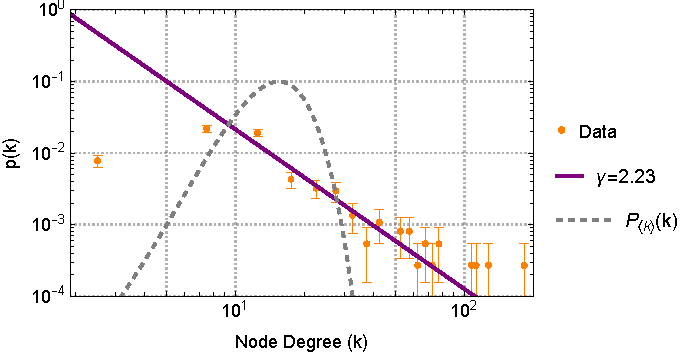
\includegraphics[width=\textwidth]{assets/degreePlotLinSpace.pdf}
         \caption{Data aggregation using linear binning. We show the best fit obtained by discarding the first two and last four points.}
         \label{fig:degree-logloglin}
     \end{subfigure}
     \hfill
     \begin{subfigure}[h]{\linewidth}
         \centering
         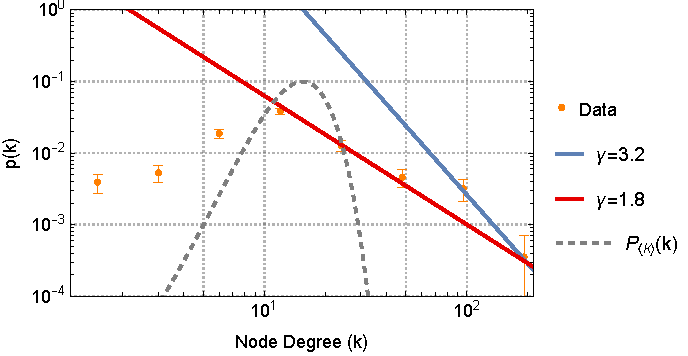
\includegraphics[width=\textwidth]{assets/degreePlotLogLog.pdf}
         \caption{Data aggregation using logarithic binning. Two possible fits are shown: one which takes into consideration only the last two points (blue) and one which takes into consideration the last five points (red). The latter has a value of $\gamma = 1.8$ which is anomalous (see section \ref{subsec:scale-free})   }
         \label{fig:degree-logloglog}
     \end{subfigure}
     \caption{Node degree distribution and fitting. The first plot (a) used linear binning to aggregate the data, while the second plot (b) used logarithmic binning. The results are different and, moreover, the values of $\gamma$ obtained in (b) are anomalous. When fitting these distribution, it is advised to use logarithmically-spaced bins; in this scenario, I believe the results which I obtained by using linearly-spaced bins are more reliable. In both plots, the dashed gray line is the best fit for a Poisson distribution (null hypothesis).  }
     \label{fig:degree-loglog}
\end{figure}


\subsection{Scale-free property}
\label{subsec:scale-free}
By definition \cite{barabasi}, a scale-free network is a network whose degree distribution follows a power law; that is:
\begin{equation}
    p(k) = C k^{-\gamma}.
    \label{eq:scale-law}
\end{equation}

In Nature we find that scale-free networks emerge in a wide variety of systems, such as: the internet \cite{barabasi99}, protein networks \cite{barabasi21}, metabolic networks \cite{barabasi20} and e-mail networks \cite{barabasi113}. The importance of scale-free networks arises from the fact that they exhibit some universal properties, that can be characterized solely by the exponent $\gamma$.
The main difference between a scale-free and a random network lies in the high-$k$ tail of the distribution. This difference is illustrated in \autoref{fig:degree-loglog}: here, we can see that the probability of finding a high-degree node in a scale-free networks is by orders of magnitude higher than in a random network. These high-degree nodes are often called \emph{hubs} and their existence plays a crucial role in determining both the robustness of a network and its small-world properties.
In \autoref{fig:degree-plot} I have shown how the node degrees are spatially distributed for the Trainline network. From this plot, it is easy to see that there are many, high-degree hubs spread troughout the whole network (they coincide with the busiest cities, as intuitively one would expect).

\begin{figure}[h]
    \centering
    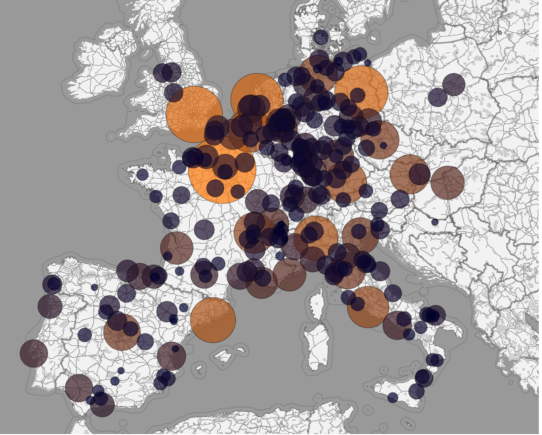
\includegraphics[width=1\linewidth]{report/assets/degreePlot.pdf}
    \caption{
    Visualization of the node degree distribution. The high-degree hubs correspond to European capitals and major cities. Each circle's color and size scale with the degree of its respective node.
}
    \label{fig:degree-plot}
\end{figure}

\subsubsection{Meaning of scale-free}
The origin of the term \emph{scale-free} comes from the fact that, for certain values of $\gamma$, the moments $\langle p(k)^n \rangle$ of the distribution \eqref{eq:scale-law} diverge if $n > 1$. Since the expectation value for a random variable $k$ exhibits fluctuations on the order of $\sqrt{\langle k^2 \rangle}$, having this value diverge would mean that, if we were to choose a node at random, we could expect it to be both arbitrarily small or large. This is in contrast to what we find for random networks, where the second moment is $\langle k^2 \rangle = \langle k \rangle^2$ and thus, the fluctuations are on the order of $\sqrt{\langle k \rangle}$. While in the latter case the average degree quantifies a scale for the fluctuations, in the former we cannot really define a scale due to the divergence of the second moment.

\subsubsection{(Ultra) small world properties}
\label{subsec:gammas}
Many of the properties of a scale-free network depend on the value of the exponent $\gamma$.
In this section, I will briefly discuss how $\gamma$ influences the \emph{small-world} property of a network; that is, the comparatively slower scaling of the average diameter $\langle d \rangle$ of a network with respect to its number of nodes. In other words, a network is said to exhibit small-world properties if the average distance between two nodes is relatively small, even if the number of nodes is very large. In the next sections, I will also show how the robustness properties of a scale-free network depend on $\gamma$.
A more in-depth explaination of these results can be found in \cite{barabasi}, and all of them can be obtained analytically \cite{barabasi120, barabasi121}.

\begin{itemize}
    \item $\gamma < 2$: \textbf{anomalous regime (\rom 1)}. Real, large networks cannot really follow this scaling law, as for $\gamma > 2$ we have that $\langle k \rangle$ diverges for large N. This would imply that the degree of the largest hub grows faster than the size of the network, which is not possible by definition.
    
    \item $\gamma = 2$: \textbf{anomalous regime (\rom 2)}. In this regime, we have that $\langle d \rangle \sim \text{constant}$. This means that the degree of the largest hub is approximately equal to the number of nodes in the network. This forces the network into a \emph{hub-and-spoke} configuration, in which all nodes are connected to a single, centralized hub.

    \item $2 < \gamma < 3$: \textbf{ultra-small world/scale free regime}. Here, we have that $\langle 
    d \rangle \sim \log{}\log N$; moreover, the first moment of $k$ converges, but all of the other moments diverge. In this regime, we find the presence of many high-degree hubs that are connected to small-degree nodes. This phenomenon effectively shrinks the distance between all the nodes of the network.

    \item $\gamma = 3$: \textbf{critical point}. Here $\langle d \rangle \sim \frac{\log N}{\log{} \log N}$, which is slower than the ultra-small wold regime but faster than the small-world regime.

    \item $\gamma > 3$: \textbf{small world/random network regime}. Here, $\langle d \rangle \sim \log N$ and $\langle k^2 \rangle$ converges. Hubs continue to exist, but they are not sufficiently large to make a significant difference with respect to a random network of the same size.
\end{itemize}

\subsection{Discussion of the fit results}
The proportionality constant $C$ of \eqref{eq:scale-law} can be obtained by imposing the normalization condition:
\begin{equation*}
    \sum _{k=1}^{+\infty} p(k) = 1.
\end{equation*}
Node degrees can only assume discrete values but, if we consider the limit in which the number of nodes is large, we can switch to the continuum formalism and compute $C$ more easily:
\begin{equation}
    \begin{aligned}
        C &= \frac{1} {\int_{k_{\min}}^{+\infty} k^{-\gamma} dk} \\
          &= (\gamma -1) k_{\min} ^{\gamma-1},    
    \end{aligned}
    \label{eq:kmin}
\end{equation}
where $k_{\min}$ is the smallest degree for which we expect the power law \eqref{eq:scale-law} to hold. The values of $k_{\min}$ and $\gamma$ can then be found by performing a fit on the data; the proper methodology can be found on \cite{barabasi}.

By plugging the fit result obtained in the previous section into \eqref{eq:kmin}, we obtain the estimate: $k_{\min} = 2.42$ and $\gamma=2.23$, which corresponds to the ultra-small world regime discussed in section \ref{subsec:gammas}.
This result is exactly what we would expect to obtain from a good transport network: the ultra-small world property implies that any node (city) can be reached in a short time by any other node, even if the two nodes considered are small, scarcely-connected cities.
Moreover, if we compute the mean graph distance of the Trainline network we obtain $\langle d \rangle = 2.28$, which is comparable to $\log{} \log N = 1.70$, as discussed in section \ref{subsec:gammas}. Graphically, we can get an idea of how the ultra-small world effect comes into play by looking at \autoref{fig:betweenness-plot}. There, I have plotted the \emph{betweennes centrality} $g(v)$ of each node $v$, which is a property related to the number of shortest paths that pass through it:
\begin{equation*}
    g(v) = \sum_{i \neq v \neq j} \frac{\sigma_{ij}(v)}{\sigma_{ij}},
\end{equation*}
where $\sigma_{ij}(v)$ is the number of shortest paths from $i$ to $j$ that pass through $v$ and $\sigma_{ij}$ is the number of all shortest paths from $i$ to $j$.
The nodes with very high betweenness centrality represent the hubs which are responsible for shortening the distances across the network.

At least one previous work \cite{gamma4} has run the same analysis on a similar European train network \cite{woodcock}, but they obtained a different result of $\gamma = 4.11$. The discrepancy of these results most likely comes from the different natures of the networks considered.

\begin{figure}
    \centering
    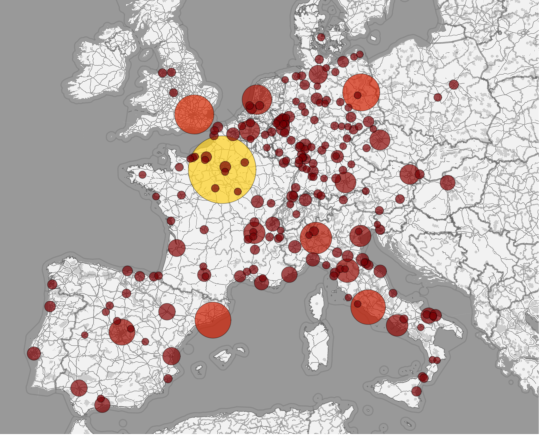
\includegraphics[width=1\linewidth]{report/assets/communitiesPlot.pdf}
    \caption{    Visualization of the node betweenness centrality distribution. The nodes with highest centrality correspond to European capitals and major cities. Each circle's color and size scale with the betweenness centrality of its respective node.}
    \label{fig:betweenness-plot}
\end{figure}

\section{Degree correlations}
Degree correlations quantify the likelihood of a high-degree node to connect to a low-degree node and vice-versa. They appear in many real-world networks (such as, the Internet, biological networks and social networks \cite{barabasi}), but not in all of them (e.g. the power grid does not exhibit degree correlations \cite{barabasi}). The study of degree correlation can help shed light on some network properties; 
for the scope of this work, what concerns us is the relation between degree correlations and network robustness.

\subsection{Possible cases}
We can distinguish three possible types of networks:
\begin{enumerate}
    \item \textbf{Neutral networks}. If there is no degree correlation, we say that a network is neutral. This is true, for example, in random networks.
    \item \textbf{Assortative networks}. This is the case if there is positive correlation between node degrees. In these types of networks, high-degree nodes tent to link to other high-degree nodes, and small-degree nodes to other small-degree nodes.
    \item \textbf{Disassortative networks}. This is the case if there is negative correlation between node degrees. Here, high-degree nodes tent to connect to low-degree nodes and vice-versa. 
\end{enumerate}

If the nodes of a network start randomly failing, we expect to see a phase transition at around some value of $\langle k \rangle$ for which the size of the giant component of the network falls to zero. Assortativity delays the phase transition in the following way:
\begin{itemize}
    \item In assortative networks, the phase transition happens at a lower value of $\langle k \rangle$, meaning that a higher number of nodes must fail in order to lose the giant component.
    \item In disassortative network, the opposite is true, meaning that the network will break up after a smaller number of nodes is removed.
\end{itemize}

\subsection{Measuring correlations}
Mathematically, all the information about degree correlation is contained in the \emph{degree correlation matrix} $e_{ij}$, which is defined as:
\begin{align*}
    e_{ij} = \text{Probability of finding nodes with degrees }\\ i \text{ and } j \text{ at the end of a randomly selected link.}
\end{align*}
One can compute \cite{barabasi} $e_{ij}$ explicitly for random networks. The result is:
\begin{equation*}
    e_{ij} = q_i q_j,
\end{equation*}
where $q_k$ is the probability of finding a node of degree-k at the end of a randomly selected link, given by
\begin{equation*}
    q_k = \frac{k\ p(k)} {\langle k \rangle}.
\end{equation*}
From an operative standpoint, working using $e_{ij}$ directly is quite cumbersome and thus, it is better to introduce the \emph{degree correlation function}:
\begin{equation*}
    k_{nn}(k) = \sum_{k'}k'P(k'|k).
\end{equation*}
$P(k'|k)$ is the probability to reach a degree-$k'$ node by following a link from a degree-$k$ node and thus $k_{nn}(k)$is the average degree of the neighbors of all degree-$k$ nodes.

The assortativity of a network depends on $k_{nn}(k)$ in the following way:
\begin{itemize}
    \item For neutral netowrks, we expect it to be a constant: $k_{nn}(k) = \langle k^2\rangle / \langle k\rangle$.
    \item For assortative networks, we expect it to follow a positive trend: $\frac d {dk} k_{nn}(k) > 0$.
    \item For disassortative networks, we expect the opposite: $\frac d {dk}k_{nn}(k) < 0$.
\end{itemize}

\subsection{Results from the data}
I have plotted the degree-correlation matrix in \autoref{fig:degree-corr-matrix} and, more importantly, the trend of the degree correlation function in \autoref{fig:corr-function}. From the latter, it is immediate to see that the data follows a downward trend; this means that the network is disassortative and thus more vulnerable to failures. Again, this result is not compatible with the one obtained in \cite{gamma4}, in which their network was observed to be assortative.

\begin{figure}[h]
    \centering
    \begin{subfigure}[h]{\linewidth}
        \centering
        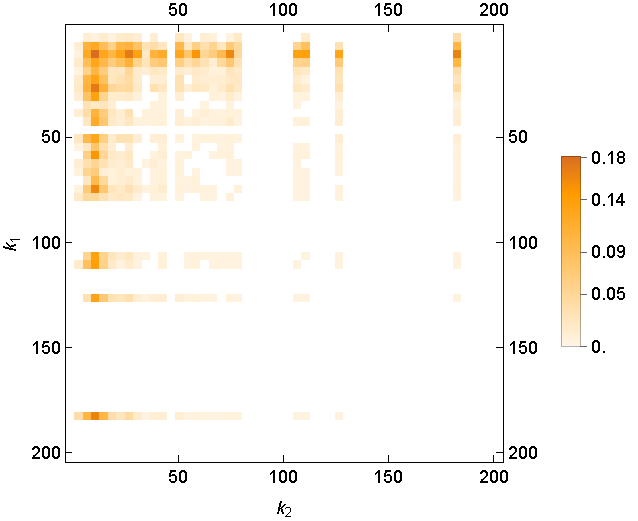
\includegraphics[width=.98\linewidth]{report/assets/assortativityMatrix.pdf}
        \caption{Degree correlation matrix}
        \label{fig:degree-corr-matrix}
    \end{subfigure}
    \hfill
    \begin{subfigure}[h]{\linewidth}
        \centering
        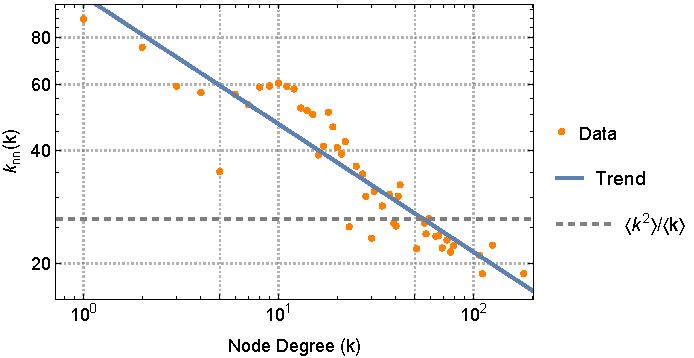
\includegraphics[width=1\linewidth]{report/assets/assortativityPlot.pdf}
        \caption{Trend for the degree correlation function. The fit indicates a downwards trend that follows the power law $\sim k^{-.34}$.}
        \label{fig:corr-function}
    \end{subfigure}
        \caption{Results of the degree correlation analysis: degree correlation matrix (a) and fit result for the degree correlation function (b).}
    \label{fig:assortativity}
\end{figure}